\section{Discussion}

\subsection{Answering Research Questions}
\subsubsection{RQ1}
Do the popular DFR tools (as available in the market) meet the NIST CFTT standards? 
If not, which tool meets which part of the standard? 

Generally, we found that the DFR tools we tested did not meet the NIST CFTT standards.
Testdisk\cite{testdisk} failed to fulfill core feature 1 because it did not identify deleted files in two test cases.
All tools fulfilled core feature 2, as they produced a recovered object for every deleted file they identified.
Autopsy\cite{autopsy} and Magnet AXIOM\cite{axiom} failed to fulfill core feature 3 because in several test cases they did not recover data they had access to.
All tools failed to fulfill core feature 4 because in many cases they recovered data which was not part of the original file.

\subsubsection{RQ2}
What factors make the tools fail or succeed?

The most common factor causing tools to fail is when a deleted file has been overwritten.
Core feature 4 requires that a tool only recover data which was originally a part of the deleted file.
A tool's success regarding this feature is thus a measure of its restraint.
The only tool to consistently fulfill core feature 4 is FTK Imager.\cite{ftk}
When it detects that a file has been partially or completely overwritten by another file, it omits the deleted sections (and everything after them in FAT).
However, in cases when the overwriting file has also been deleted, even FTK fails to fulfill this core feature.
It is worth noting that Autopsy does appear to react to overwritten files; for some cases of overwriting in FAT, it returns only a single cluster, presumably the starting cluster of the deleted file.
However, since that cluster has been overwritten, Autopsy still fails to fulfill core feature 4 in those cases.

Another factor that causes multiple failures is simulated in FAT cases 8, 9, and 10.
In FAT, a file can be written starting close to the end of the file system, without enough space to fit contiguously.
In such cases, the file must be fragmented, and since it is already at the end of the file system, the second fragment will appear closer to the beginning of the file system (this is illustrated in Figure \ref{fig:case_8}).
This scenario could realistically occcur when the file system is almost full.
In these cases, no tool is able to recover the second fragment of the deleted file; however, because FAT fragmentation is unpredictable, we only require them to recover the first fragment.
Interestingly, Autopsy and Magnet AXIOM fail to recover anything at all, with Autopsy returning a short file of null data, and Magnet AXIOM returning an empty file after displaying an error message.

\subsubsection{RQ3}
Are the free DFR tools more effective compared to the enterprise-level (proprietary) tools?

As can be observed in Figure \ref{fig:results_table}, no type of tool clearly outperforms the others.
FTK Imager, a proprietary enterprise-level tool, passes the most test cases by a large margin.
However, the other enterprise-level tool, Magnet AXIOM, passes the least test cases.
Given the available data, we cannot reach a definite conclusion for RQ3.

\begin{figure}[h]
    \begin{tabular}{| c | c | c |}
    \hline
    \textbf{DFR Tool} &  \textbf{Type} &  \textbf{Passes} \\ \hline
    Autopsy & free open source & 5 \\ \hline
    TestDisk & free open source & 10 \\ \hline
    Recuva & proprietary freemium & 7 \\ \hline
    FTK Imager & proprietary enterprise & 18 \\ \hline
    Magnet AXIOM & proprietary enterprise & 4 \\ \hline
    \end{tabular}
    
    \caption{DFR tools sorted by type. ``Passes'' refers to the number of test cases in which a tool fulfills all 4 core features.}
    \label{fig:results_table}
\end{figure}

\subsection{Ambiguity in Standards}
While determining how to interpret the NIST standards, we encountered ambiguities in their current wording.

\subsubsection{Core Feature 3 and FAT Fragmentation}
Core feature 3's requirement that a tool recover ``all non-allocated data blocks identified in a residual metadata entry''\cite{meta:dfr:standards} is not well-defined when considering a FAT file system. 
In FAT, the only relevant metadata left over after file deletion is the address of the first cluster of file data, and the file's length. 
If the deleted file is fragmented at any point, no evidence remains in the metadata. 
Therefore, interpreting the wording very closely, a tool is only required to recover the first cluster of a file's data. 
As this would not be particularly useful, it is unlikely that this was the intended meaning. 
For these tests we interpret core feature 3 as requiring the first contiguous segment of unallocated clusters starting from the first cluster originally allocated to the deleted file. 
In other words, if the file is fragmented, the tool must recover at least the first fragment. 
If a file is partially overwritten, the tool must recover at least the clusters before the overwritten part.
In essense, the tool is only required to recover data for which it does not have to guess what file the data belongs to.
However, it should be emphasized this is an assumption and the intent of the standard in this case needs clarification.

\subsubsection{Contradictory Core Features}
When designing test cases, we found situations in which core features 3 and 4 are entirely incompatible. 
Core feature 3 specifies ``all non-allocated data blocks identified in a residual metadata entry,''\cite{meta:dfr:standards} but that can sometimes still include data from other files. 
One such situation is when a deleted file is overwritten, and then the overwriting file is also deleted, such as in case 5i (as seen in Figure \ref{fig:case_5i}).

\begin{figure}[h]
    \centering
    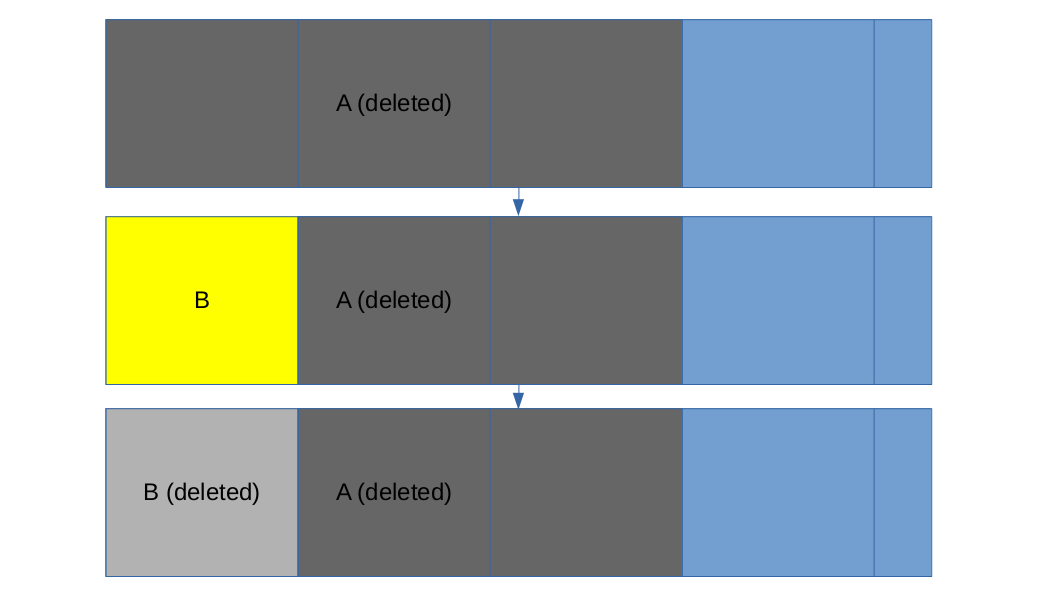
\includegraphics[width=\linewidth]{fig/case5i.png}
    \caption{Test Case 5i}
    \label{fig:case_5i}
\end{figure}

Assuming the file system is NTFS (to avoid the afforementioned ambiguity with core feature 3 and FAT), the residual metadata entry for File A (in this case its Master File Table entry) should list every cluster File A once occupied. 
All of those clusters are unallocated, so to fulfill core feature 3, the tool must recover them. 
However, some of those clusters have been overwritten by File B. Core feature 4 requires that a tool only recover ``data blocks from the Deleted Block Pool,''\cite{meta:dfr:standards} and defines the Deleted Block Pool as all blocks which ``have not been reallocated or reused.''\cite{meta:dfr:standards}
Core feature 3 would require tools to recover the clusters reused by File B, while core feature 4 would forbid this. 
It could be argued that the tool should use File B's metadata to recognize that File B overwrote File A, but this is not always realistic. 
While the file system stores information such as creation and modification times, this is not ``essential metadata,'' meaning it is not involved in the operation of the file system, so operating systems may implement it inconsistently, or not at all.\cite{carrier:filesystems}
Since the time information cannot be counted on to be reliable, there is no way to know for sure which file overwrote which. 
It is also possible for File B's metadata entry to be overwritten at some point before File A's, in which event there is no way for the tool to know File B even existed.

The standards document acknowledges that the ``potential for corruption [is] inherent with data that is no longer maintained by a file system,''\cite{meta:dfr:standards} and that the recovered object ``may not completely match the original FS-Object.''\cite{meta:dfr:standards}
We propose the standards themselves should be revised to better account for such situations.
This would most likely mean adding an exception to either the third or fourth core feature, for cases in which data blocks are overwritten and subsequently deallocated.
